
\subsubsection{Critical Parameters for Superconductivity}
Critical current:
\begin{equation}
    I_\text{c}(T) = I \frac{T-T_\text{cs}}{T_\text{c}-T_\text{cs}}
\end{equation}
\\
Critical temperature:
\begin{equation}
    T_\text{c}(B) = 9.2 \cdot [1- \frac{B}{14.5}]^{0.59}~\text{for}~B~<~10~\text{T}
\end{equation}
\\
Critical magnetic field: 
\begin{equation}
    B_\text{c2}(T) = B_\text{c2}(T=0) \cdot [1-(\frac{T}{T_\text{c}(B=0)})^{n}],
\end{equation}
where
$B_\text{c2}(T=0)=14.5~\text{T}$, $T_\text{c}(B=0)=9.2~\text{K}$, $n=1.7$.

\subsubsection{Current Flow in Copper Matrix}

Current sharing temperature: 
\begin{equation}
    T_\text{cs} = T_\text{c} (1 - \frac{I}{\text{c}_1 + \text{c}_2 B }),
\end{equation}
where $\text{c}_1=3449~\text{A}$ and $\text{c}_2=-257~\text{AT}^{-1}$
\\
Current in copper matrix: 
\begin{equation}
    \left\{ \begin{array}{lll}
    I_\text{Cu} = 0 & \text{for}~T < T_\text{cs} \\ \\
    I_\text{Cu} = I - I_\text{c} & \text{for}~T_\text{cs} \leq T<T_\text{c}  \\ \\
    I_\text{Cu} = I & \text{for}~T_\text{cs} \leq T
    \end{array} \right.
\end{equation}
\\
Joule heating: 
\begin{equation}
    \left\{ \begin{array}{lll}
    q_\text{Joule} = 0 & \text{for}~T < T_\text{cs} \\ \\
    q_\text{Joule} = \rho_\text{Cu}(T, B) \frac{(I-I_\text{c})^2}{{\text{a}_\text{Cu}}^2}& \text{for}~T_\text{cs} \leq T<T_\text{c}  \\ \\
    q_\text{Joule} = \rho_\text{Cu}(T, B) \frac{I^2}{{\text{a}_\text{Cu}}^2} & \text{for}~T_\text{cs} \leq T
    \end{array} \right.
\end{equation}

\begin{figure}[ht!]
\centering
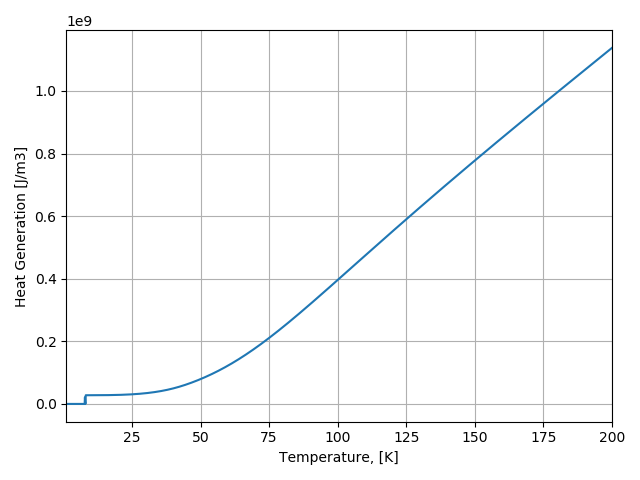
\includegraphics[width=0.49\linewidth]{figures/skew_quad_bcs/magnetic_field_mapping/Heat_Generation_Curve_B_3.png}
\caption{Heat Generation Curve as a function of temperature for B=3 T}
\label{fig:H_gen_curve}
\end{figure}